\chapter{CNN}
\section{Teori}
\subsection{Teks Tokenizer}
Untuk memudahkan mesin memahami maksud dari apa yang kita inginkan dalam machine learning, kata pada teks disebut token, dan proses vektorisasi dari bentuk kata ke dalam token tersebut disebut tokenizer dan tokenizer akan merubah sebuah teks menjadi simbol, kata, ataupun biner dan bentuk lainnya kedalam token. Untuk lebih jelasnya perhatikan ilustrasi berikut. Disini saya mempunyai sebuah kalimat yaitu "Nama Saya Tasya Wiendhyra" maka ketika kita lakukan proses tokenizer maka akan berubah menjadi ['Nama', 'Saya', 'Tasya', 'Wiendhyra].

\subsection{konsep dasar K Fold Cross Validation pada dataset komentar Youtube} 
\begin{lstlisting}[caption=K Fold Cross Validation,label={lst:7.0}]
kfold = StratifiedKFold(n_splits=5)
splits = kfold.split(d, d['CLASS'])
\end{lstlisting}

StartifiedKFold berisikan presentasi sampel untuk setiap kelas. Dimana dalam ilustrasi ini sampel dibagi menjadi 5 dalam setiap class nya. Kemudian sampel tadi akan dimasukan kedalam class dari dataset youtube tadi.

Untuk ilustrasi lebih jelasnya, ada pada gambar berikut :
\begin{figure}[ht]
\centering
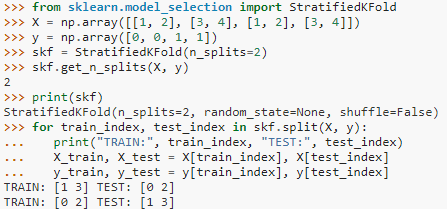
\includegraphics[scale=0.5]{figures/Chapter 7/1164086/Teori/chapter7tasya1.PNG}
\caption{Ilustrasi KFold Cross Tasya}
\label{Teori}
\end{figure}

\subsection{kode program for train, test in splits} 
Maksudnya yaitu untuk menguji apakah setiap data pada dataset sudah di split dan tidak terjadi penumpukan. Yang dimana maksudnya di setiap class tidak akan muncul id yang sama. Ilustrasinya misalkan kita memiliki 4 baju dengan model yang berbeda. Kemudian kita bagikan kedua anak, tentunya setiap anak yang menerima baju tidak memiliki baju yang sama modelnya.

\subsection{Jelaskan apa maksudnya kode program \emph{train\_content = d['CONTENT'].iloc[train\_idx]} dan \emph{test\_content = d['CONTENT'].iloc[test\_idx]}. dilengkapi dengan ilustrasi atau gambar}

Maksudnya yaitu mengambil data pada kolom atau index CONTENT yang merupakan bagian dari train\_idx dan test\_idx. Ilustrasinya, ketika data telah diubah menjadi train dan test maka kita dapat memilihnya untuk ditampilkan pada kolom yang diinginkan.

\subsection{Soal No. 5 Jelaskan apa maksud dari fungsi \emph{tokenizer = Tokenizer(num\_words=2000)} dan \emph{tokenizer.fit\_on\_texts(train\_content)}, dilengkapi dengan ilustrasi atau gambar} 
Dimana variabel tokenizer akan melakukan vektorisasi kata menggunakan fungsi Tokenizer yang dimana jumlah kata yang ingin diubah kedalam bentuk token adalah 2000 kata. Dan untuk \emph{tokenizer.fit\_on\_texts(train\_content)} maksudnya kita akan melakukan fit tokenizer hanya untuk dat trainnya saja tidak dengan data test nya untuk kolom CONTENT. Ilustrasinya, Jadi, jika Anda memberikannya sesuatu seperti, "Kucing itu duduk di atas tikar." Ini akan membuat kamus s.t. word\_index ["the"] = 0; word\_index ["cat"] = 1 itu adalah kata -> kamus indeks sehingga setiap kata mendapat nilai integer yang unik.

\subsection{Jelaskan apa maksud dari fungsi \emph{d\_train\_inputs = tokenizer.texts\_to\_matrix(train\_content, mode='tfidf')} dan \emph{d\_test\_inputs = tokenizer.texts\_to\_matrix(test\_content, mode='tfidf')}, dilengkapi dengan ilustrasi kode dan atau gambar} 


Maksudnya yaitu untuk variabel d\_train\_inputs akan melakukan tokenizer dari bentuk teks ke matrix dari data train\_content dengan mode matriksnya yaitu tfidf begitu juga dengan variabel d\_test\_inputs untuk data test. Berikut gambar ilustrasinya
\begin{figure}[ht]
\centering
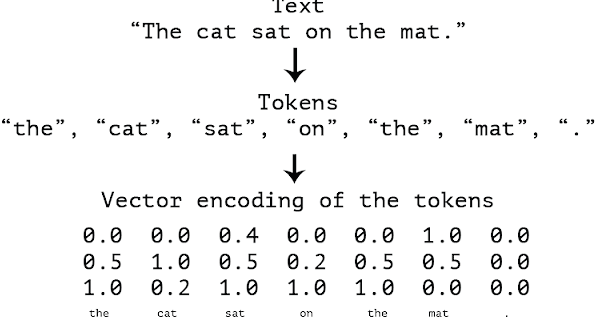
\includegraphics[scale=0.5]{figures/Chapter 7/1164086/Teori/chapter7tasya2.png}
\caption{Ilustrasi Text To Matrix Tasya}
\label{Teori}
\end{figure}

\subsubsection{Jelaskan apa maksud dari fungsi \emph{d\_train\_inputs = d\_train\_inputs/np.amax(np.absolute(d\_train\_inputs))} dan \emph{d\_test\_inputs = d\_test\_inputs/np.amax(np.absolute(d\_test\_inputs))}, dilengkapi dengan ilustrasi atau gambar}

Fungsi tersebut akan membagi matrix tfidf tadi dengan amax yaitu mengembalikan maksimum array atau maksimum sepanjang sumbu. Yang hasilnya akan dimasukan kedalam variabel d\_train\_inputs untuk data train dan d\_test\_inputs untuk data test dengan nominal absolut atau tanpa ada bilangan negatif dan koma.
\begin{figure}[ht]
\centering
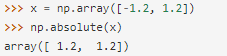
\includegraphics[scale=0.5]{figures/Chapter 7/1164086/Teori/chapter7tasya4.png}
\caption{Ilustrasi np Absolute Tasya}
\label{Teori}
\end{figure}

\subsubsection{Jelaskan apa maksud fungsi dari \emph{d\_train\_outputs = np\_utils.to\_categorical(d['CLASS'].iloc[train\_idx])} dan \emph{d\_test\_outputs = np\_utils.to\_categorical(d['CLASS'].iloc[test\_idx])} dalam kode program, dilengkapi dengan ilustrasi atau gambar}

Dalam variabel d\_train\_output dan d\_test\_outputs akan dilakukan one hot encoding, dimana np\_utilsakan mengubah vektor dengan bentuk integer ke matriks kelas biner untuk kolom CLASS dimana nantinya hanya akan ada dua pilihan yaitu 1 atau 0. 1 untuk spam 0 untuk non spam atau sebaliknya. Berikut gambar ilustrasinya :
\begin{figure}[ht]
\centering
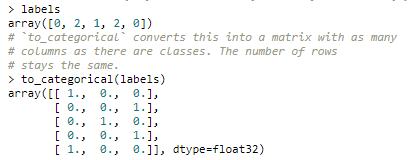
\includegraphics[scale=0.5]{figures/Chapter 7/1164086/Teori/chapter7tasya5.png}
\caption{Ilustrasi One Hot Encoding Tasya}
\label{Teori}
\end{figure}

\subsubsection{Jelaskan apa maksud dari fungsi di listing \ref{lst:7.1}. Gambarkan ilustrasi Neural Network nya dari model kode tersebut.}
\begin{lstlisting}[caption=Membuat model Neural Network,label={lst:7.1}]
       model = Sequential()
       model.add(Dense(512, input_shape=(2000,)))
       model.add(Activation('relu'))
       model.add(Dropout(0.5))
       model.add(Dense(2))
       model.add(Activation('softmax'))
\end{lstlisting}
Penjelasannya sebagai berikut :
\begin{itemize}
\item Melakukan pemodelan Sequential
\item Layer pertama dense dari 512 neuron untuk inputan dengan inputan tadi yang sudah dijadikan matriks sebanyak 2000
\item Activationnya menggunakan fungsi relu yaitu jika ada inputan dengan nilai maksimum maka inputan itu yang akan terpilih.
\item Dropout ini untuk melakukan pembobotan, dimana pembobotan hanya dilakukan 50\% saja agar tidak terjadi penumpukan data dari dense inputan tadi
\item Dense 2 mengkategorikan 2 neuron untuk output nya yaitu 1 dan 0.
\item Untuk dense diatas aktivasinya menggunakan fungsi Softmax.
\end{itemize}

Ilustrasinya seperti berikut :
\begin{figure}[ht]
\centering
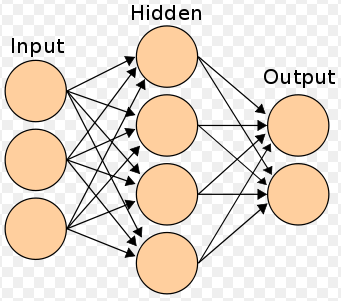
\includegraphics[scale=0.5]{figures/Chapter 7/1164086/Teori/chapter7tasya6.png}
\caption{Ilustrasi Neural Network Pemodelan Tasya}
\label{Teori}
\end{figure}

\subsubsection{Jelaskan apa maksud dari fungsi di listing \ref{lst:7.2} dengan parameter tersebut}
\begin{lstlisting}[caption=Compile model,label={lst:7.2}]
	model.compile(loss='categorical_crossentropy', optimizer='adamax',
	                  metrics=['accuracy'])
\end{lstlisting}
Melakukan peng compile-an dari model Sequential tadi dengan Loss yandengang merupakan fungsi optimisasi skor  menggunakan categorical\_crossentropy , dan menggunakan algoritma adam sebagai optimizer. Adam yaitu algoritma pengoptimalan yang dapat digunakan sebagai ganti dari prosedur penurunan gradien stokastik klasik untuk memperbarui bobot jaringan yang berulang berdasarkan data training.Dengan metrik yaitu fungsi yang digunakan untuk menilai kinerja mode Anda disini menggunakan fungsi accuracy.

\subsubsection{Jelaskan apa itu Deep Learning}
Deep Learning  adalah subbidang machine learning yang berkaitan dengan algoritma yang terinspirasi oleh struktur dan fungsi otak yang disebut jaringan saraf tiruan atau Artificial Neural Networks. Jaringan saraf tiruan, algoritma yang terinspirasi oleh otak manusia, belajar dari sejumlah besar data. Demikian pula dengan bagaimana kita belajar dari pengalaman, algoritma pembelajaran yang mendalam akan melakukan tugas berulang kali, setiap kali sedikit mengubahnya untuk meningkatkan hasilnya.

\subsubsection{Jelaskan apa itu Deep Neural Network, dan apa bedanya dengan Deep Learning}
Deep Neural Network adalah jaringan syaraf tiruan (JST) dengan beberapa lapisan antara lapisan input dan output. DNN menemukan manipulasi matematis yang benar untuk mengubah input menjadi output, apakah itu hubungan linear atau hubungan non-linear. Merupakan jaringan syaraf dengan tingkat kompleksitas tertentu, jaringan syaraf dengan lebih dari dua lapisan. Deep Neural Network menggunakan pemodelan matematika yang canggih untuk memproses data dengan cara yang kompleks.

DNN hanya terdiri dari dua laipsan yaitu input dan output, sedangkan dalam Deep learning kita dapat mendefiniskan layer sebanyak yang kita inginkan atau butuhkan.

\subsubsection{Jelaskan dengan ilustrasi gambar buatan sendiri(langkah per langkah) bagaimana perhitungan algoritma konvolusi dengan ukuran stride (NPM mod3+1) x (NPM mod3+1) yang terdapat max pooling}
Stridenya 3
\begin{itemize}
\item terdapat data seperti berikut 
\begin{figure}[ht]
\centering
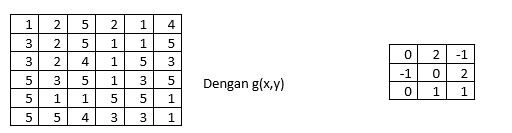
\includegraphics[scale=0.5]{figures/Chapter 7/1164086/Teori/chapter7tasya7.png}
\caption{Algoritma Konvulusi Tasya}
\label{Teori}
\end{figure}
\item Kemudian hitung konvolusi untuk setiap matriksnya seperti berikut :
\begin{itemize}
\item pertama
\begin{figure}[ht]
\centering
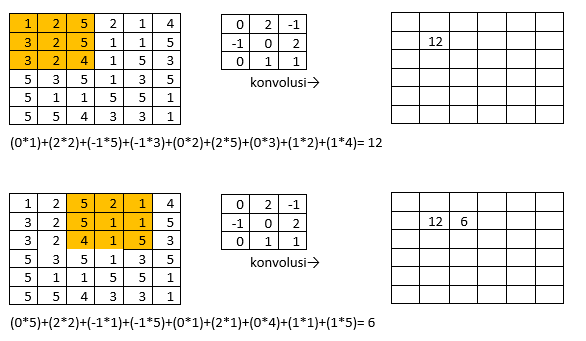
\includegraphics[scale=0.5]{figures/Chapter 7/1164086/Teori/chapter7tasya8.png}
\caption{Algoritma Konvulusi Tasya}
\label{Teori}
\end{figure}
\item Kedua
\begin{figure}[ht]
\centering
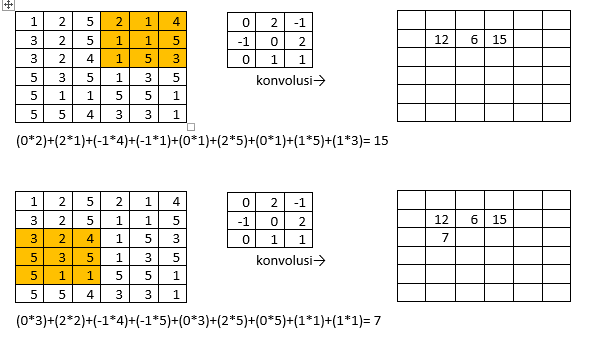
\includegraphics[scale=0.5]{figures/Chapter 7/1164086/Teori/chapter7tasya9.png}
\caption{Algoritma Konvulusi Tasya}
\label{Teori}
\end{figure}
\item Ketiga
\begin{figure}[ht]
\centering
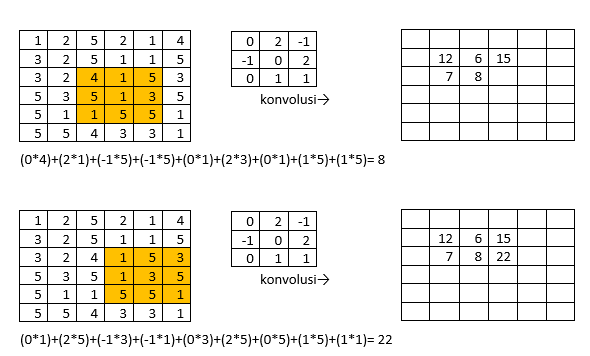
\includegraphics[scale=0.5]{figures/Chapter 7/1164086/Teori/chapter7tasya10.png}
\caption{Algoritma Konvulusi Tasya}
\label{Teori}
\end{figure}
\item Keempat
\begin{figure}[ht]
\centering
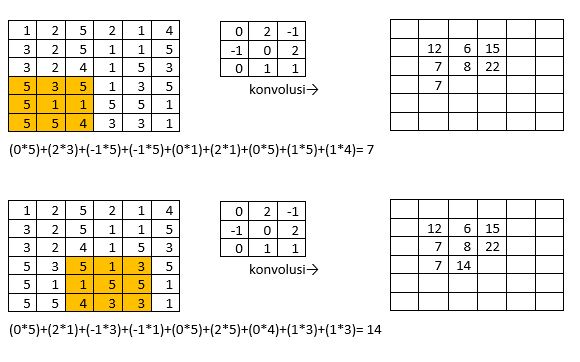
\includegraphics[scale=0.5]{figures/Chapter 7/1164086/Teori/chapter7tasya11.png}
\caption{Algoritma Konvulusi Tasya}
\label{Teori}
\end{figure}
\item Kelima
\begin{figure}[ht]
\centering
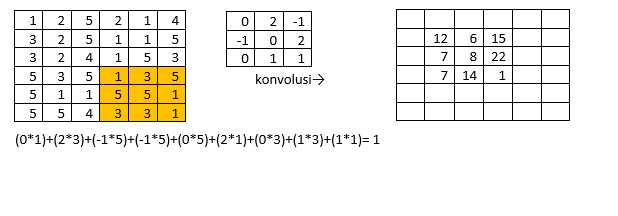
\includegraphics[scale=0.5]{figures/Chapter 7/1164086/Teori/chapter7tasya12.png}
\caption{Algoritma Konvulusi Tasya}
\label{Teori}
\end{figure}
\end{itemize}
\item Didapatkan hasil akhir nilai konvolusi dan juga max poolingnya seperti berikut
\begin{figure}[ht]
\centering
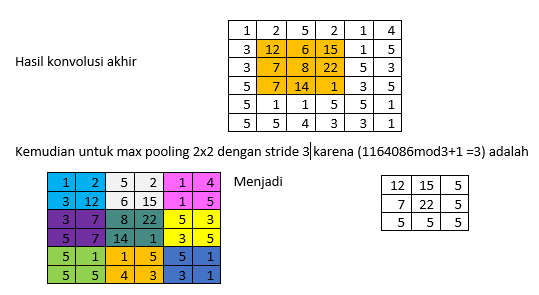
\includegraphics[scale=0.5]{figures/Chapter 7/1164086/Teori/chapter7tasya13.png}
\caption{Algoritma Konvulusi Tasya}
\label{Teori}
\end{figure}
\end{itemize}


\subsection{Praktek}
\subsubsection{No.1 Kode Program Blok \# In 1}
\lstinputlisting[language=python, firstline=8, lastline=20]{src/Chapter7/1164086/in1.py}
Keterangannya sebagai berikut :
\begin{itemize}
\item Pertama kita akan mengimpor librari csv
\item Dimana dari librai PIL atau Pillow atau Python Imaging Library akan diimpor modul Image yang di inisiasikan sebagain pil\_image. Modul Image menyediakan kelas dengan nama yang sama yang digunakan untuk mewakili gambar PIL. Modul ini juga menyediakan sejumlah fungsi pabrik, termasuk fungsi untuk memuat image dari file, dan untuk membuat image baru.
\item mengimpor librari image dari keras .Yang menghasilkan kumpulan data gambar tensor dengan augmentasi data waktu nyata. Data akan diulang (dalam batch). 
\item Berikut Hasilnya :
\begin{figure}[ht]
\centering
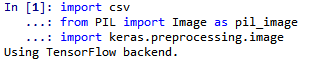
\includegraphics[scale=0.5]{figures/Chapter 7/1164086/Praktek/chapter7tasya14.png}
\caption{Kode Program Blok In 1 Tasya}
\label{Praktek}
\end{figure}
\end{itemize}

\subsubsection{No.2 Kode Program Blok \# In 2}
\lstinputlisting[language=python, firstline=8, lastline=20]{src/Chapter7/1164086/in2.py}
Keterangannya sebagai berikut :
\begin{itemize}
\item variabel imgs berisikan array kosong
\item Variabel classes berisikan array kosong
\item Membuka file csv dari Folder HSYv2 dengan nama file hasy-data-labels.csv sebagai csvfile
\item Variabel csvreader akan menggunakan fungsi reader pada library csv untuk membaca file csv tadi yang disimpan di csvfile.
\item Dimana variabel i dimuali dari nol.
\item Untuk setiap baris pada  csvreader
\item Jika i lebih besar dari 0
\item Jadi itu akan mengambil contoh Gambar PIL dan mengubahnya menjadi array numpy dengan mengambil data dari HSYv2 dan dimulai dari baris ke nol.
\item Hasil dari variabel img akan dibagi dengan 255.0
\item .append akan membuat list array baru untuk baris 0 baris 2 pada img.
\item Menyimpan setiap class nya  pada baris 2
\item Penambahan i sebanyak 1. 
\item Hasilnya seperti berikut :
\begin{figure}[ht]
\centering
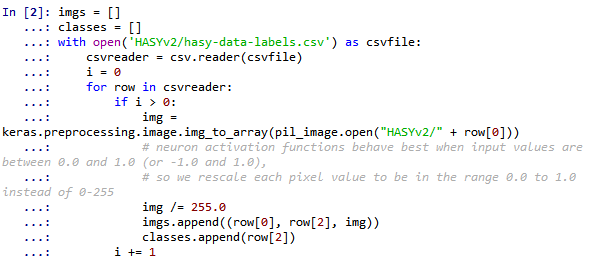
\includegraphics[scale=0.5]{figures/Chapter 7/1164086/Praktek/chapter7tasya15.png}
\caption{Kode Program Blok In 2 Tasya}
\label{Praktek}
\end{figure}
\end{itemize}

\subsubsection{No.3 Kode Program Blok \# In 3}
\lstinputlisting[language=python, firstline=8, lastline=20]{src/Chapter7/1164086/in3.py}
Keterangannya sebagai berikut :
\begin{itemize}
\item Impor librari Random dari Python
\item Melakukan pengacakan untuk imgs dengan Metode Shuffle  untuk mengocok urutan di tempat. yaitu, mengubah posisi item dalam daftar.
\item Membagi data dari imgs dengan cara mengalikan 80\% dengan jumlah data dari imgs.
\item Untuk data train mengambil hasil dari perhitungan sebelumnya.
\item Untuk data test mengambil sisa dari jumlah yang telah dijadikan data train
\item Hasilnya seperti berikut :
\begin{figure}[ht]
\centering
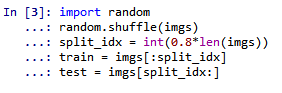
\includegraphics[scale=0.5]{figures/Chapter 7/1164086/Praktek/chapter7tasya16.png}
\caption{Kode Program Blok In 3 Tasya}
\label{Praktek}
\end{figure}
\end{itemize}

\subsubsection{No.4 Kode Program Blok \# In 4}
\lstinputlisting[language=python, firstline=8, lastline=20]{src/Chapter7/1164086/in4.py}
Keterangannya sebagai berikut :
\begin{itemize}
\item Impor librari Numpy yang di inisiasikan sebagai np
\item Variabel train\_input mengubah input menjadi sebuah array yang diambil dari baris 2, data train.
\item Variabel test\_input mengubah input menjadi sebuah array yang diambil dari baris 2, data test.
\item Variabel train\_output mengubah input menjadi sebuah array yang diambil dari baris 1, data train.
\item Variabel train\_output mengubah input menjadi sebuah array yang diambil dari baris 1, data test.
\item Hasilnya seperti berikut 
\begin{figure}[ht]
\centering
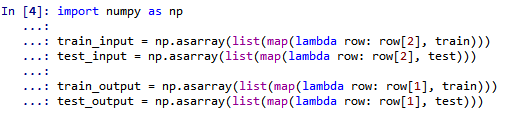
\includegraphics[scale=0.5]{figures/Chapter 7/1164086/Praktek/chapter7tasya17.png}
\caption{Kode Program Blok In 4 Tasya}
\label{Praktek}
\end{figure}
\end{itemize}

\subsubsection{No.5 Kode Program Blok \# In 5}
\lstinputlisting[language=python, firstline=8, lastline=20]{src/Chapter7/1164086/in5.py}
Keterangannya sebagai berikut :
\begin{itemize}
\item Impor Fungsi LabelEncoder
\item Impor Fungsi OneHotEncoder
\item Berikut hasilnya :
\begin{figure}[ht]
\centering
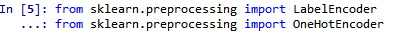
\includegraphics[scale=0.5]{figures/Chapter 7/1164086/Praktek/chapter7tasya18.png}
\caption{Kode Program Blok In 5 Tasya}
\label{Praktek}
\end{figure}
\end{itemize}

\subsubsection{No.6 Kode Program Blok \# In 6}
\lstinputlisting[language=python, firstline=8, lastline=20]{src/Chapter7/1164086/in6.py}
Keterangannya sebagai berikut :
\begin{itemize}
\item Variabel label\_encoder akan memanggil fungsi LabelEncoder tadi.
\item variabel integer\_encoded akan menggunakan labelencoder untuk melakukan fit pada classes agar berubah datanya menjadi integer.
\item Berikut hasilnya :
\begin{figure}[ht]
\centering
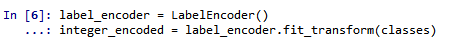
\includegraphics[scale=0.5]{figures/Chapter 7/1164086/Praktek/chapter7tasya19.png}
\caption{Kode Program Blok In 6 Tasya}
\label{Praktek}
\end{figure}
\end{itemize}

\subsubsection{No.7 Kode Program Blok \# In 7}
\lstinputlisting[language=python, firstline=8, lastline=20]{src/Chapter7/1164086/in7.py}
Keterangannya sebagai berikut :
\begin{itemize}
\item Variabel onehot\_encoder akan memanggil fungsi OneHotEncoder dimana tidak berisikan matriks sparse.
\item Pada variabel integer\_encoded akan diubah bentuknya dimana setiap nilai integer akan direpresentasikan sebagai vektor binari dengan nilai 0 kecuali index dari integer tersebut ditandai dengan 1.
\item Melakukan fit untuk one hot encoder kedalam integer\_encoder.
\item Berikut hasilnya :
\begin{figure}[ht]
\centering
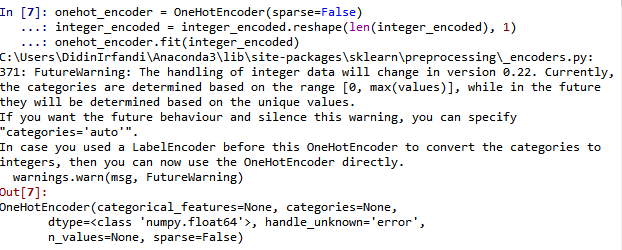
\includegraphics[scale=0.5]{figures/Chapter 7/1164086/Praktek/chapter7tasya20.png}
\caption{Kode Program Blok In 7 Tasya}
\label{Praktek}
\end{figure}
\end{itemize}

\subsubsection{No.8 Kode Program Blok \# In 8}
\lstinputlisting[language=python, firstline=8, lastline=20]{src/Chapter7/1164086/in8.py}
Keterangannya sebagai berikut :
\begin{itemize}
\item Variabel train\_output\_int  akan mengubah data dari train\_output menjadi LabeEncoder
\item Dimana pada train\_output setelah diubah labelnya menjadi integer dilakukan one hot encoding diambil dari train\_output\_int dan menggunakan .reshape untuk memberikan bentuk baru ke array tanpa mengubah datanya dengan keterangan jika index dari integer tersebut ditandai dengan 1 dan sisanya yang bukan nol.
\item Variabel test\_output\_int  akan mengubah data dari test\_output menjadi LabeEncoder
\item Dimana pada train\_output setelah diubah labelnya menjadi integer dilakukan one hot encoding diambil dari test\_output\_int dan menggunakan .reshape untuk memberikan bentuk baru ke array tanpa mengubah datanya dengan keterangan jika index dari integer tersebut ditandai dengan 1 dan sisanya yang bukan nol.
\item Variabel num\_classes akan menampilakn jumlah data dari classes yang telah dilakukan label encoder
\item Menampilkan tulisan "Number of classes : \%d dmana mengembalikan nilai integer dari num\_classes.
\item Hasilnya sebagai berikut : 
\begin{figure}[ht]
\centering
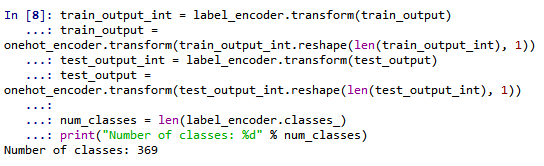
\includegraphics[scale=0.5]{figures/Chapter 7/1164086/Praktek/chapter7tasya21.png}
\caption{Kode Program Blok In 8 Tasya}
\label{Praktek}
\end{figure}
\end{itemize}

\subsubsection{No.9 Kode Program Blok \# In 9}
\lstinputlisting[language=python, firstline=8, lastline=20]{src/Chapter7/1164086/in9.py}
Keterangannya sebagai berikut :
\begin{itemize}
\item Impor Sequential dari model pada librari Keras.
\item Impor Dense, Dropout, Flatten dari modul Layers pada librari Keras.
\item Impor Conv2D, MaxPooling2D dari modul Layers pada librari Keras.
\item Hasilnya seperti berikut : 
\begin{figure}[ht]
\centering
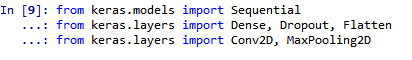
\includegraphics[scale=0.5]{figures/Chapter 7/1164086/Praktek/chapter7tasya22.png}
\caption{Kode Program Blok In 9 Tasya}
\label{Praktek}
\end{figure}
\end{itemize}

\subsubsection{No.10 Kode Program Blok \# In 10}
\lstinputlisting[language=python, firstline=8, lastline=20]{src/Chapter7/1164086/in10.py}
Keterangannya sebagai berikut :
\begin{itemize}
\item Melakukan pemodelan Sequential.
\item Menambahkan Konvolusi 2D dengan 32 filter konvolusi masing-masing berukuran 3x3 dengan algoritam activation relu dengan data dari train\_input mulai dari baris nol.
\item Menambahkan Max Pooling dengan matriks 2x2.
\item Dilakukan lagi penambahkan Konvolusi 2D dengan 32 filter konvolusi masing-masing berukuran 3x3 dengan algoritam activation relu.
\item Menambahkan lagi Max Pooling dengan matriks 2x2.
\item Mendefinisikan inputan dengan 1024 neuron dan menggunakan algoritma tanh untuk activationnya.
\item Dropout terdiri dari pengaturan secara acak tingkat pecahan unit input ke 0 pada setiap pembaruan selama waktu pelatihan, yang membantu mencegah overfitting sebesar 50\% .
\item Untuk output layer menggunakan data dari variabel num\_classes dengan fugsi activationnya softmax.
\item Mengonfigurasi proses pembelajaran, yang dilakukan melalui metode compile,sebelum melatih suatu model.
\item Menampilkan atau mencetak representasi ringkasan model yang telah dibuat.
\item Hasilnya sebagai berikut :
\begin{figure}[ht]
\centering
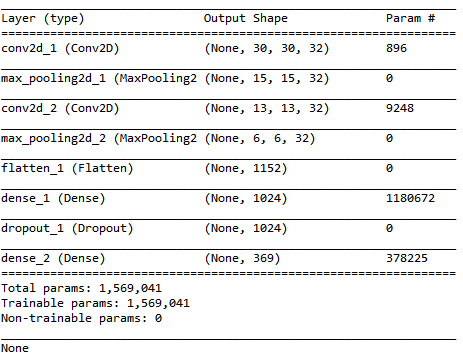
\includegraphics[scale=0.5]{figures/Chapter 7/1164086/Praktek/chapter7tasya23.png}
\caption{Kode Program Blok In 10 Tasya}
\label{Praktek}
\end{figure}
\end{itemize}

\subsubsection{No.11 Kode Program Blok \# In 11}
\lstinputlisting[language=python, firstline=8, lastline=20]{src/Chapter7/1164086/in11.py}
Keterangannya sebagai berikut :
\begin{itemize}
\item Impor Modul Callbacks dari Librari Keras.
\item Variabel callback mendefinisikan Callback ini untuk menulis log untuk TensorBoard, yang memungkinkan Anda untuk memvisualisasikan grafik dinamis dari pelatihan dan metrik pengujian Anda, serta histogram aktivasi untuk berbagai lapisan dalam model Anda.
\item Hasilnya sebagai berikut : 
\begin{figure}[ht]
\centering
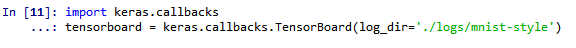
\includegraphics[scale=0.5]{figures/Chapter 7/1164086/Praktek/chapter7tasya24.png}
\caption{Kode Program Blok In 11 Tasya}
\label{Praktek}
\end{figure}
\end{itemize}

\subsubsection{No.12 Kode Program Blok \# In 12}
\lstinputlisting[language=python, firstline=8, lastline=20]{src/Chapter7/1164086/in12.py}
Keterangannya sebagai berikut :
\begin{itemize}
\item Melakukan fit model dengan 32 ukuran subset dari sampel pelatihan Anda
\item Epoch sebanyak 10 kali
\item Vebrose=2 maksudnya menampilkan nomor dari epoch yang sedang berjalan atau yang sudah dijalankan.
\item Validasi plit sebanayk 20\% sebagai fraksi data pelatihan untuk digunakan sebagai data validasi.
\item Menggunakan TensorBoard sebagai callback untuk diterapkan selama pelatihan dan validasi.
\item Variabel score mengembalikan nilai evaluate untuk menampilkan data lost dan data accuracy dari test
\item Menampilkan data loss dengan menghitung jumlah kemunculan nol .
\item Menampilkan data accuracy dengan menghitung jumlah kemunculan 1.
\item Berikut hasilnya :
\begin{figure}[ht]
\centering
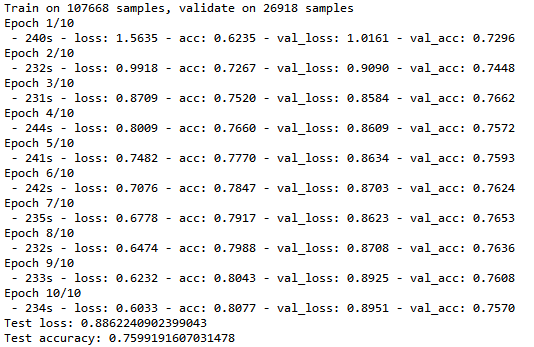
\includegraphics[scale=0.5]{figures/Chapter 7/1164086/Praktek/chapter7tasya25.png}
\caption{Kode Program Blok In 12 Tasya}
\label{Praktek}
\end{figure}
\end{itemize}

\subsubsection{No.13 Kode Program Blok \# In 13}
\lstinputlisting[language=python, firstline=8, lastline=20]{src/Chapter7/1164086/in13.py}
Keterangannya sebagai berikut :
\begin{itemize}
\item impor modul time dari python anaconda
\item Variabel result berisikan array kosong.
\item Menggunakan convolution 2D yang dimana akan memiliki 1 atau 2 layer.
\item Mendefinisikan dense\_size dengan ukuran 128, 256, 512, 1024, 2048
\item Mendefinsikan drop\_out dengan 0, 25\%, 50\%, dan 75\%
\item Melakukan pemodelan Sequential
\item Jika ini adalah layer pertama, kita perlu memasukkan bentuk input.
\item Kalau tidak kita hanya akan menambahkan layer.
\item Kemudian, setelah menambahkan layer konvolusi, kita akan melakukan hal yang sama dengan max pooling.
\item  Lalu, kita akan meratakan atau flatten dan menambahkandense size ukuran apa pun yang berasal dari dense\_size. Dimana akan selalu menggunakan algoritma tanh
\item Jika dropout digunakan, kita akan menambahkan layer dropout. Menyebut dropout ini berarti, katakanlah 50\%, bahwa setiap kali ia memperbarui bobot setelah setiap batch, ada peluang 50\% untuk setiap bobot yang tidak akan diperbarui
\item menempatkan ini di antara dua lapisan padat untuk dihidupkan dari melindunginya dari overfitting.
\item  Lapisan terakhir akan selalu menjadi jumlah kelas karena itu harus, dan menggunakan softmax. Itu dikompilasi dengan cara yang sama.
\item Atur direktori log yang berbeda untuk TensorBoard sehingga dapat membedakan konfigurasi yang berbeda.
\item Variabel start akan memanggil modul time atau waktu
\item Melakukan fit atau compile 
\item MElakukan scoring dengan .evaluate yang akan menampilkan data loss dan accuracy dari model
\item end merupakan variabel untuk melihat waktu akhir pada saat pemodelan berhasil dilakukan.
\item Menampilkan hasil dari run skrip diatas
\item Hasilnya sebagai berikut :
\begin{figure}[ht]
\centering
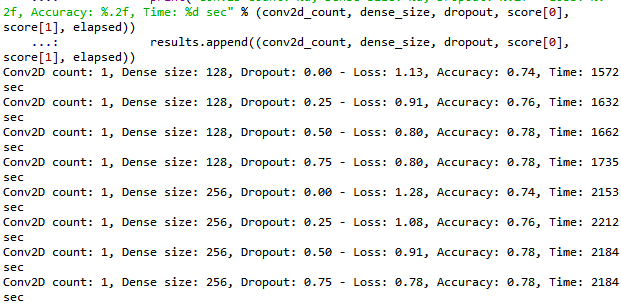
\includegraphics[scale=0.5]{figures/Chapter 7/1164086/Praktek/chapter7tasya26.png}
\caption{Kode Program Blok In 13 Tasya}
\label{Praktek}
\end{figure}
\end{itemize} 

\subsubsection{No.14 Kode Program Blok \# In 14}
\lstinputlisting[language=python, firstline=8, lastline=20]{src/Chapter7/1164086/in14.py}
Keterangannya sebagai berikut :
\begin{itemize}
\item Melakukan pemodelan Sequential
\item Untuk layer pertama, Menambahkan Convolutio 2D dengan dmensi 32, dan ukuran matriks 3x3 dengan function aktivasi yang digunakan yaitu relu dan menampilkan input\_shape
\item Dilakukan Max Pooling 2D dengan ukuran matriks 2x2
\item Untuk layer kedua, melakukan Convolusi lagi dengan kriteria yang sama tanpa menambahkan input, ini dilakukan untuk mendapatkan data yang terbaik
\item Flatten digubakan ntuk meratakan inputan
\item Menambahkan dense input sebanyak 128 neuron dengan menggunakan function aktivasi tanh.
\item Dropout sebanyak 50\% untuk menghindari overfitting
\item Menambahkan dense pada model untuk output dimana layer ini akan menjadi jumlah dari class yang ada.
\item Mengcompile model yang didefinisikan diatas
\item Menampilkan ringkasan dari pemodelan yang dilakukan
\item Gambarnya seperti berikut :
\begin{figure}[ht]
\centering
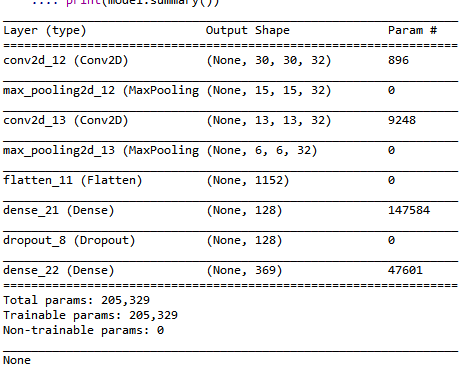
\includegraphics[scale=0.5]{figures/Chapter 7/1164086/Praktek/chapter7tasya27.png}
\caption{Kode Program Blok In 14 Tasya}
\label{Praktek}
\end{figure}
\end{itemize}

\subsubsection{No.15 Kode Program Blok \# In 15}
\lstinputlisting[language=python, firstline=8, lastline=20]{src/Chapter7/1164086/in15.py}
Keterangannya sebagai berikut :
\begin{itemize}
\item Melakukan fit dengan join data train dan test agar dapat dilakukan pelatihan untuk jaringan pada smeua data yang dimiliki.
\item Hasilnya sebagai berikut :
\begin{figure}[ht]
\centering
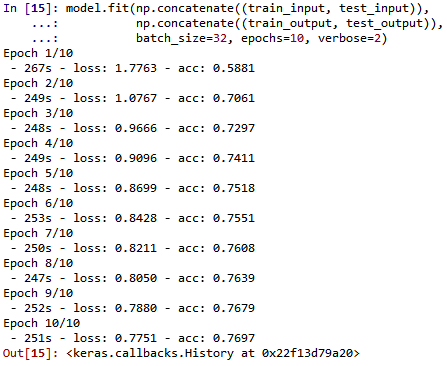
\includegraphics[scale=0.5]{figures/Chapter 7/1164086/Praktek/chapter7tasya29.png}
\caption{Kode Program Blok In 15 Tasya}
\label{Praktek}
\end{figure}
\end{itemize}

\subsubsection{No.16 Kode Program Blok \# In 16}
\lstinputlisting[language=python, firstline=8, lastline=20]{src/Chapter7/1164086/in16.py}
Keterangannya sebagai berikut :
\begin{itemize}
\item Menyimpan atau save model yang telah di latih dengan nama mathsymbols.model 
\item Hasilnya seperti berikut :
\begin{figure}[ht]
\centering
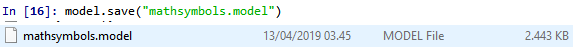
\includegraphics[scale=0.5]{figures/Chapter 7/1164086/Praktek/chapter7tasya30.png}
\caption{Kode Program Blok In 16 Tasya}
\label{Praktek}
\end{figure}
\end{itemize}

\subsubsection{No.17 Kode Program Blok \# In 17}
\lstinputlisting[language=python, firstline=8, lastline=20]{src/Chapter7/1164086/in17.py}
Keterangannya sebagai berikut :
\begin{itemize}
\item Simpan label enkoder (untuk membalikkan one-hot encoder) dengan nama classes.npy
\item Hasilnya seperti berikut :
\begin{figure}[ht]
\centering
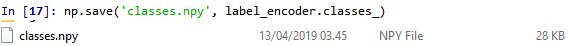
\includegraphics[scale=0.5]{figures/Chapter 7/1164086/Praktek/chapter7tasya31.png}
\caption{Kode Program Blok In 17 Tasya}
\label{Praktek}
\end{figure}
\end{itemize}

\subsubsection{No.18 Kode Program Blok \# In 18}
\lstinputlisting[language=python, firstline=8, lastline=20]{src/Chapter7/1164086/in18.py}
Keterangannya sebagai berikut :
\begin{itemize}
\item Impor models dari librari Keras
\item Variabel model2 akan memanggil model yang telah disave tadi 
\item Menampilkan ringkasan dari hasil pemodelan
\item Hasilnya sebagai berikut :
\begin{figure}[ht]
\centering
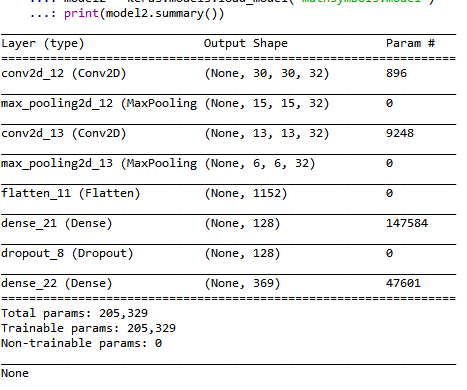
\includegraphics[scale=0.5]{figures/Chapter 7/1164086/Praktek/chapter7tasya32.png}
\caption{Kode Program Blok In 18 Tasya}
\label{Praktek}
\end{figure}
\end{itemize}

\subsubsection{No.19 Kode Program Blok \# In 19}
\lstinputlisting[language=python, firstline=8, lastline=20]{src/Chapter7/1164086/in19.py}
Keterangannya sebagai berikut :
\begin{itemize}
\item Memanggil fungsi LabelEncoder
\item Variabel label\_encoder akan memanggil class yang disave sebelumnya.
\item Function Predict akan mengubah gambar kedalam bentuk array
\item Variabel prediction akan melakukan prediksi untuk model2 dengan reshape variabel newimg dengan bentukarray 4D.
\item Variabel inverted akan mencari nilai tertinggi output dari hasil prediksi tadi
\item Menampilkan hasil dari variabel prediction dan inverted
\item Hasilnya sebagai berikut :
\begin{figure}[ht]
\centering
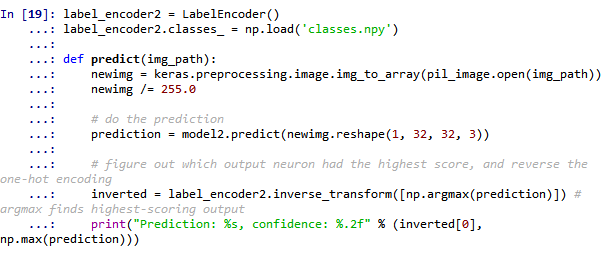
\includegraphics[scale=0.5]{figures/Chapter 7/1164086/Praktek/chapter7tasya33.png}
\caption{Kode Program Blok In 19 Tasya}
\label{Praktek}
\end{figure}
\end{itemize}

\subsubsection{No.20 Kode Program Blok \# In 20}
\lstinputlisting[language=python, firstline=8, lastline=20]{src/Chapter7/1164086/in19.py}
Keterangannya sebagai berikut :
\begin{itemize}
\item Melakukan prediksi dari pelatihan dari gambar v2-00010.png
\item Melakukan prediksi dari pelatihan dari gambar v2-00500.png
\item Melakukan prediksi dari pelatihan dari gambar v2-00700.png
\item Hasilnya sebagai berikut :
\begin{figure}[ht]
\centering
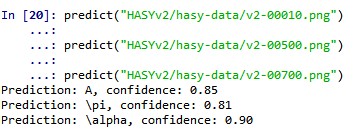
\includegraphics[scale=0.5]{figures/Chapter 7/1164086/Praktek/chapter7tasya34.png}
\caption{Kode Program Blok In 20 Tasya}
\label{Praktek}
\end{figure}
\end{itemize}

\subsection{Penanganan Error}
\subsubsection{Error Starting Kernel}
\begin{itemize}
\item Berikut merupakan screenshot error
\begin{figure}[ht]
\centering
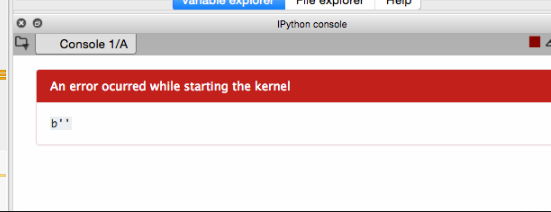
\includegraphics[scale=0.5]{figures/Chapter 7/1164086/Praktek/chapter7eror1.png}
\caption{Error Tasya}
\label{Error}
\end{figure}

\item Eror tersebut merupakan eror yang terjadi dan membuat kita tidak dapat mengakses dan menggunakan kernel atau konsol pada spyder.

\item Untuk penanganannya sebagai berikut :
\begin{enumerate}
\item Tutup spyder yang sedang dijalankan
\item Kemudian buka kembali spyder
\item Atau jika tidak berhasil, buka anaconda promt dan ketikan "conda update spyder"
\item Jika tidak berhasil juga bisa menginstall ulang anaconda
\item Maka ketika dijaalankan lagi hasilnya seperti berikut :
\begin{figure}[ht]
\centering
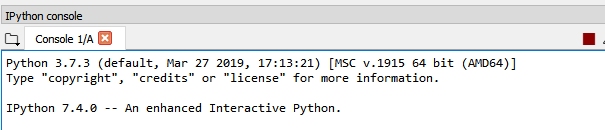
\includegraphics[scale=0.5]{figures/Chapter 7/1164086/Praktek/chapter7eror2.png}
\caption{Penanganan Error Kernel Tasya}
\label{Error}
\end{figure}
\end{enumerate}
\end{itemize}
